%=======================================================================
%  3.1  DISCOVERING & ABSTRACTING
%=======================================================================
\subsection{Discovering \& Abstracting}
\label{sec:discovering}

\subsubsection{Research path}
\label{sec:researchpath}

To find suitable solutions both the AskNature website as well as the AskNature chat were
used. The following keywords were used to find solutions produced in nature:

\begin{quote}
Cooling, thermal transfer, shading, heat reduction, reflect, evaporation
\end{quote}

Additionally the biologized questions were used to search for solutions using search
engines such as Google.

The models that were selected had to fulfill at least one function mentioned in
Section~\ref{sec:functions}. Additionally they had to fit into at least one of the defined
Life's Principles. Therefore some models were abandoned and not investigated further.

\subsubsection{Natural Models}
\label{sec:models}

\paragraph{African Elephant: Ears}
\label{sec:model_ears}

\runin{Biological mechanism}
As seen in Figure~\ref{fig:ears}, African elephants have large and highly vascularized
ears which they use as heat exchange surfaces. Warm blood is transported from the body
core into the ear, where heat is transferred to the surrounding air. By flapping their
ears additional airflow is created which further increases the heat transfer
\cite{asknature_ears}. This same approach is also used by the jackrabbit
\cite{asknature_jackrabbit}.

\begin{figure}[H]
\centering
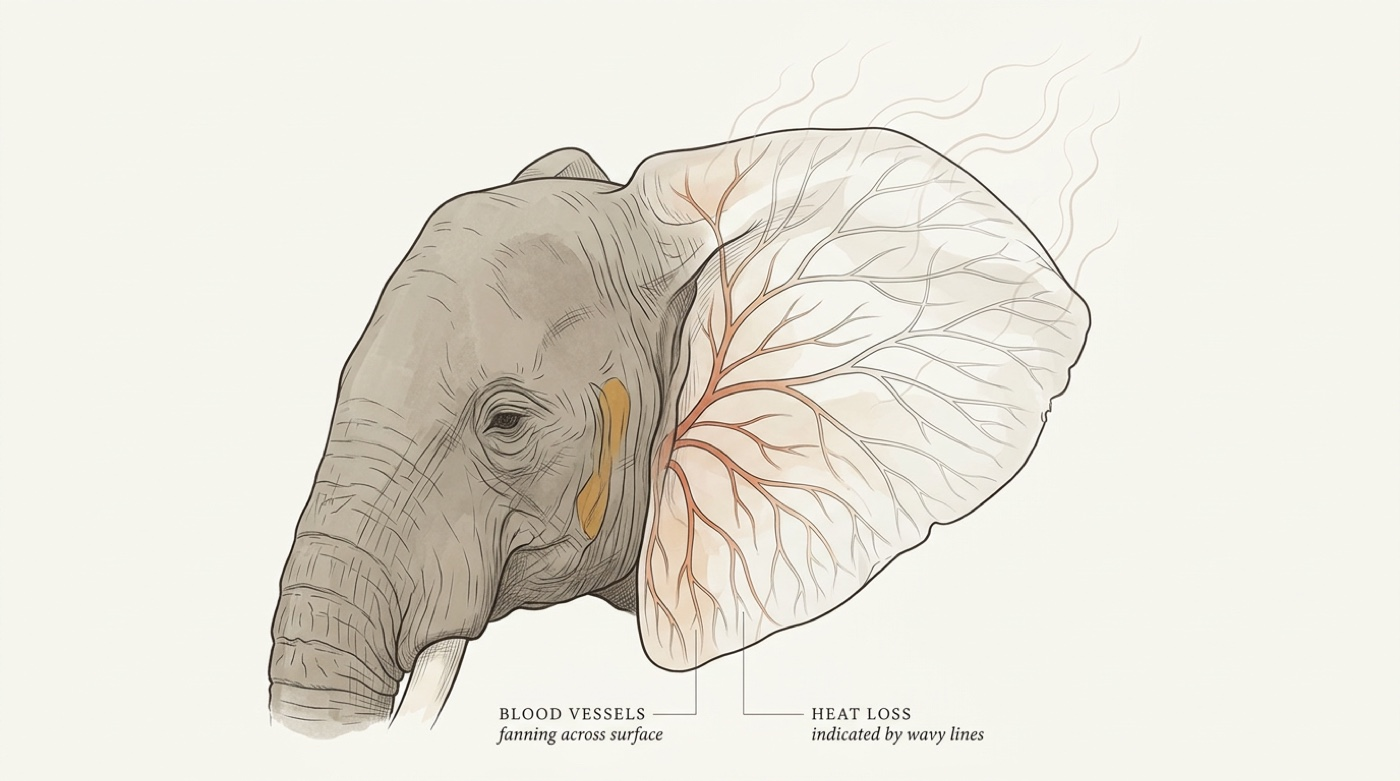
\includegraphics[width=0.72\textwidth]{figures/fig_elephant_ears.jpg}
\caption{African elephant ears (schematic illustration).}
\label{fig:ears}
\end{figure}

\runin{Functional abstraction.} Transfer thermal energy from a heat generating region to
a large exchange surface and increase airflow across this surface.

\runin{Design principle for urban cooling.} Use dedicated heat rejection surfaces in
locations with favorable airflow to transfer and dissipate heat from urban structures.

\lp{Be resource efficient / Adapt to changing conditions}

\clearpage

\paragraph{Elephant Skin: Sparse Hairs}
\label{sec:model_hair}

\runin{Biological mechanism}
African elephants have additionally to their ears a second cooling mechanism. They have
very sparsely spread hair all over their body. Due to the low density of the body hair it
does not act as an insulation layer but rather as additional surface area to transfer
heat. As seen in Figure~\ref{fig:hair}, it also serves to break the stationary air
surrounding the skin. This allows for a better heat transfer \cite{myhrvold2012}.

\begin{figure}[H]
\centering
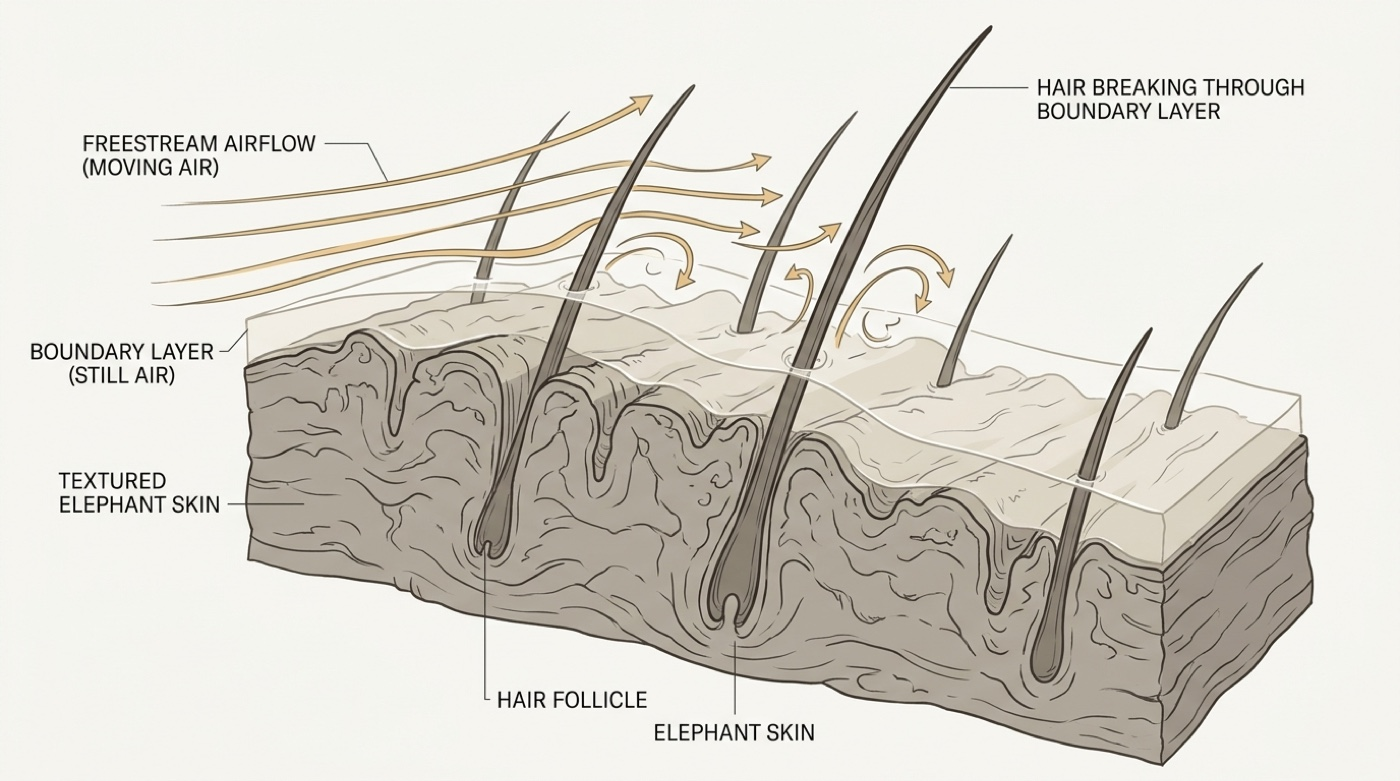
\includegraphics[width=0.72\textwidth]{figures/fig_elephant_hair.jpg}
\caption{African elephant hair (schematic illustration).}
\label{fig:hair}
\end{figure}

\runin{Functional abstraction.} Increase heat-transfer area by distributing sparse bulges
across a warm surface.

\runin{Design principle for urban cooling.} Use small surface structures on façades or
other heated urban surfaces to enhance passive heat transfer without substantially
increasing material use.

\lp{Be resource efficient}

\paragraph{Cactus Ribs}
\label{sec:model_cactus}

\runin{Biological mechanism}
Many cacti have ribbed surfaces consisting of repeated peaks and troughs. The peaks shade
parts of the troughs and therefore reduce direct solar exposure. Air within the shaded
troughs remains cooler and absorbs heat from the cactus which rises as it warms. The
ribbed geometry also increases surface area and disrupts airflow around the plant,
similar to the elephant hair \cite{asknature_cactus,lewis1977}.

\runin{Functional abstraction.} Use folded surface geometry to combine self-shading,
increased heat-transfer area and controlled interaction with airflow.

\runin{Design principle for urban cooling.} Integrate ribbed or folded geometries into
urban surfaces to reduce direct solar exposure while simultaneously promoting passive
heat dissipation.

\lp{Be resource efficient}

\clearpage

\paragraph{Saharan Silver Ant: Reflective Hairs}
\label{sec:model_ant}

\runin{Biological mechanism}
The Saharan silver ant is covered with densely packed hairs that have a triangular
cross-section and grooved surfaces. These hairs reduce heat gain in two ways: they
strongly reflect visible and near-infrared solar radiation through total internal
reflection and they increase emissivity in the mid-infrared range, allowing the ant to
radiate excess body heat more efficiently. AskNature reports that the hairs alone keep
the ant about 2\,°C cooler, while the combined mechanisms provide an additional cooling
effect of approximately 5--10\,°C \cite{asknature_anthair}.

\runin{Functional abstraction.} Use micro structured surfaces to reflect incoming solar
radiation while simultaneously enhancing thermal radiation away from the surface.

\runin{Design principle for urban cooling.} Develop façade or roof surfaces with micro
structured geometries that minimize absorption in the visible and near-infrared solar
spectrum while maximizing heat emission in the mid-infrared. This could reduce solar heat
gain and improve passive radiative cooling without requiring active energy input.

\lp{Adapt to changing conditions / Use life-friendly chemistry}

\paragraph{Desert Snail Shell}
\label{sec:model_snail}

\runin{Biological mechanism}
The desert snail \emph{Sphincterochila boissieri} limits heat gain through a highly
reflective shell and internal insulating air spaces, as seen in Figure~\ref{fig:snail}.
AskNature reports approximately 90\,\% reflectance in the visible spectrum and about
95\,\% in the near-infrared range. The snail also withdraws into the upper parts of its
shell, while air-filled spaces and limited contact with the hot substrate reduce
conductive heat transfer \cite{asknature_snail}.

\begin{figure}[H]
\centering
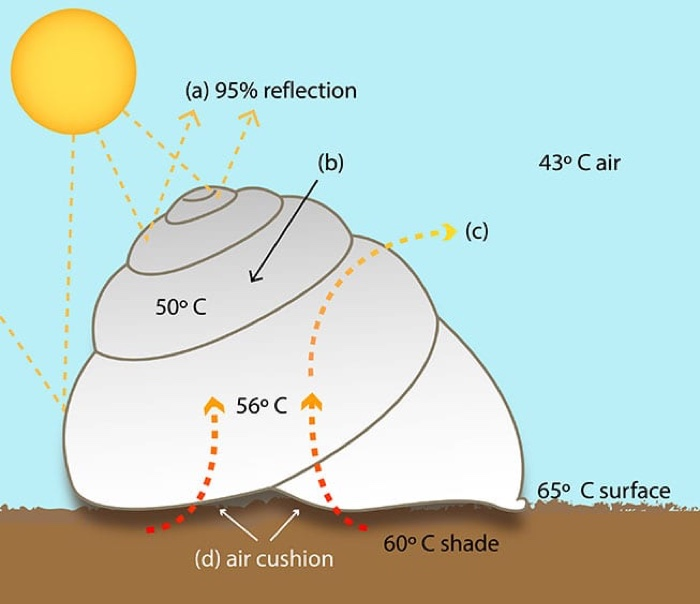
\includegraphics[width=0.55\textwidth]{figures/fig_snail.jpg}
\caption{Desert snail \cite{asknature_snail}.}
\label{fig:snail}
\end{figure}

\runin{Functional abstraction.} Reduce incoming radiant energy and interrupt conductive
heat transfer using reflective surfaces and stationary air layers.

\runin{Design principle for urban cooling.} Combine highly reflective external surfaces
with insulating or ventilated air cavities to limit solar heat storage in roofs and
façades.

\lp{Be resource efficient / Adapt to changing conditions}

\paragraph{Morpho Butterfly Wing}
\label{sec:model_morpho}

\runin{Biological mechanism}
Morpho butterflies generate their characteristic color using transparent chitin-and-air
structures at micro- and nanoscale. As seen in Figure~\ref{fig:morpho}, ridges and
cross-ribs interact with incoming light through diffraction and interference, causing
selected wavelengths to be strongly reflected. The color therefore results primarily from
physical structure rather than pigmentation \cite{asknature_morpho}.

\begin{figure}[H]
\centering
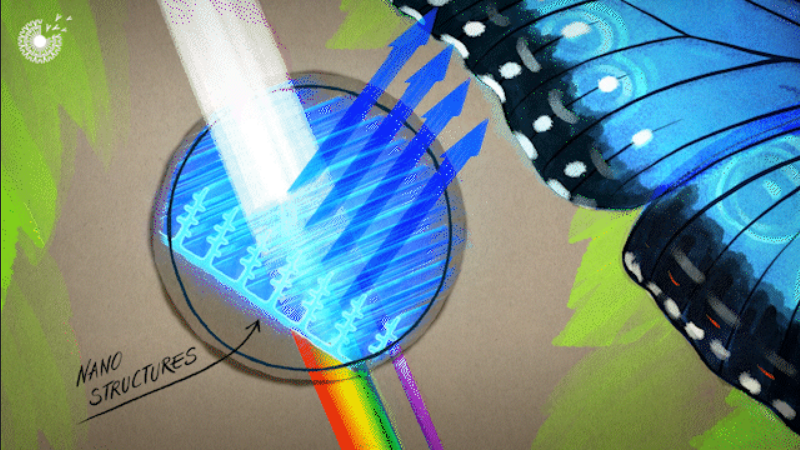
\includegraphics[width=0.75\textwidth]{figures/fig_morpho.png}
\caption{Reflection with nano structures \cite{giraldo2016}.}
\label{fig:morpho}
\end{figure}

\runin{Functional abstraction.} Control the spectral interaction between a surface and
incoming radiation through micro- and nanoscale geometry.

\runin{Design principle for urban cooling.} Engineer structured surfaces that selectively
manipulate incident solar radiation while maintaining desired optical properties. It
needs to be mentioned that the Morpho demonstrates structural color rather than
near-infrared heat rejection and that a cooling application requires separate
verification.

\lp{Be resource efficient}

\clearpage

\paragraph{Camel Fur and Sweat}
\label{sec:model_camel}

\runin{Biological mechanism}
Dromedary camels combine insulation with evaporative cooling. Figure~\ref{fig:camel}
displays how exactly this mechanism works. The sweat glands release water which removes
the body heat through evaporation, while the thick fur blocks the hot air from reaching
the skin. Furthermore the camel reflects light with its pale color \cite{asknature_camel}.

\begin{figure}[H]
\centering
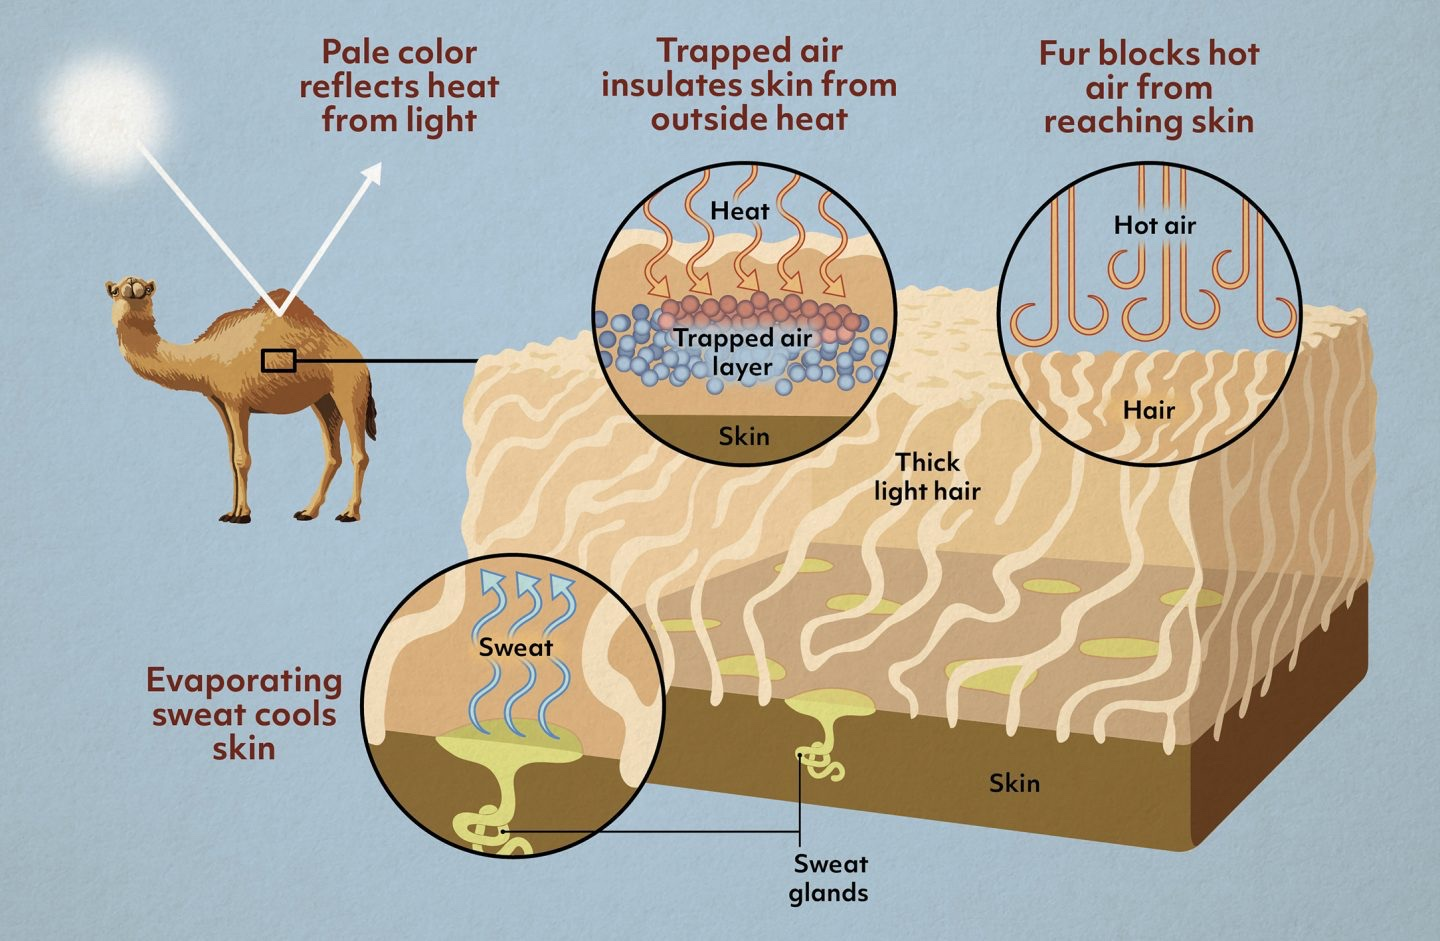
\includegraphics[width=0.75\textwidth]{figures/fig_camel.jpg}
\caption{Insulation with evaporative cooling \cite{asknature_camel}.}
\label{fig:camel}
\end{figure}

\runin{Functional abstraction.} Block heat using insulation in combination with
evaporation as a means of heat dissipation.

\runin{Design principle for urban cooling.} Combine shading or thermal insulation with
controlled evaporative cooling so that less water is required to achieve the desired
cooling effect.

\lp{Be resource efficient / Adapt to changing conditions / Use life-friendly chemistry}

\paragraph{Pine Cone Scales}
\label{sec:model_pinecone}

\runin{Biological mechanism}
Pine cone scales respond to humidity despite containing no muscles or active control
system. Their layered structure contains materials with different swelling behavior.
When moisture is absorbed, one layer expands more than the other, causing the scale to
bend and close. As the scale dries, it returns towards its open state. The movement is
reversible \cite{dawson1997}.

\runin{Functional abstraction.} Convert an environmental change directly into mechanical
movement through differential material expansion.

\runin{Design principle for urban cooling.} Use environmentally responsive material
layers to create self-actuating shading or ventilation elements that operate without
motors or electronic control.

\lp{Adapt to changing conditions / Use life-friendly chemistry}

\clearpage

\paragraph{Honeybee Fanning Thresholds}
\label{sec:model_bees}

\runin{Biological mechanism}
Western honeybee colonies regulate nest temperature through the combined behavior of
many workers. Individual bees have different temperature-response thresholds. As nest
temperature increases, progressively more bees begin ventilating the hive. This
distributed response prevents excessive system-wide reactions to small temperature
fluctuations and stabilizes the nest with no central control \cite{peters2019}.

\runin{Functional abstraction.} Distribute different activation thresholds across
multiple independent elements to create a gradual system-level response.

\runin{Design principle for urban cooling.} Use multiple passive cooling elements with
different trigger conditions so that cooling capacity increases progressively with
thermal load instead of operating through a single on/off threshold.

\lp{Be resource efficient / Adapt to changing conditions}
